\documentclass[a4paper,10pt]{report}

\usepackage{graphicx}
\usepackage{color}

\usepackage{caption}
\usepackage{subcaption}

\usepackage[portuguese]{babel}
\usepackage[utf8]{inputenc}
\usepackage[T1]{fontenc}

\usepackage{geometry}
\geometry{a4paper}
\usepackage[parfill]{parskip}

\usepackage{changepage}

\usepackage{amsmath}

\usepackage{fancyhdr}

\usepackage{nopageno}

\graphicspath{{./imagens/}}

\usepackage{url}

\usepackage{verbatim}
\usepackage{fancyvrb}

\usepackage[colorlinks=true,linkcolor=blue,citecolor=blue]{hyperref}

\usepackage{listings}
\renewcommand{\lstlistingname}{Código}
\usepackage{color}
\definecolor{grey}{rgb}{0.9,0.9,0.9}
\definecolor{greyD}{rgb}{0.5,0.5,0.5}

\lstnewenvironment{code}[1][]%
{
   \noindent
   \lstset{
	language=java,
	float=htpb,
	backgroundcolor=\color{grey},
	basicstyle=\scriptsize,
	numbers=left,
	numbersep=5pt,
	numberstyle=\tiny\color{greyD},
	breaklines=true,
	frame=single,
	#1}
}
{}

\begin{document}

\begin{titlepage}
\begin{center}

\begin{flushleft}

\includegraphics[height=3.00cm]{EENG.jpg}\\
\end{flushleft}

\vspace{2cm}

\Large{\textbf{LEI --- Licenciatura de Engenharia Informática}}\\
\vspace{1cm}
\Large{\textbf{UC8204P1 --- Programação Orientada a Objectos}}\\

\vspace{2.5cm}

\Huge{\textbf{FitnessUM}} \\

\vspace{2cm}

\Large{\textbf{Grupo XXXX}}\\
\vspace{0.5cm}
\normalsize{\textbf{Rui Camposinhos - a72625, Rui Oliveira - a67661, André Santos - a61778}}\\
\vspace{0.5cm}
\begin{figure}[h]
\centering
\begin{subfigure}{.2\textwidth}
  \centering
  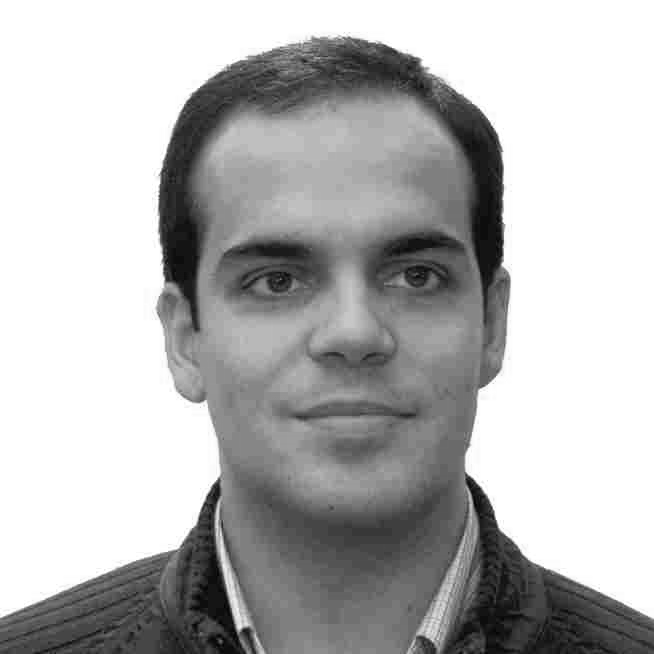
\includegraphics[width=\textwidth]{Camposinhos.jpg}
\end{subfigure}
\begin{subfigure}{.2\textwidth}
  \centering
  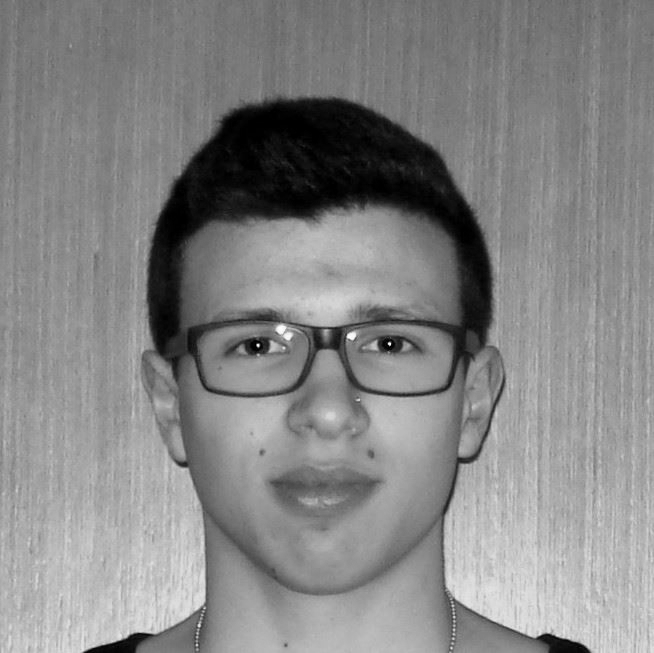
\includegraphics[width=\textwidth]{Oliveira.jpg}
\end{subfigure}
\begin{subfigure}{.2\textwidth}
  \centering
  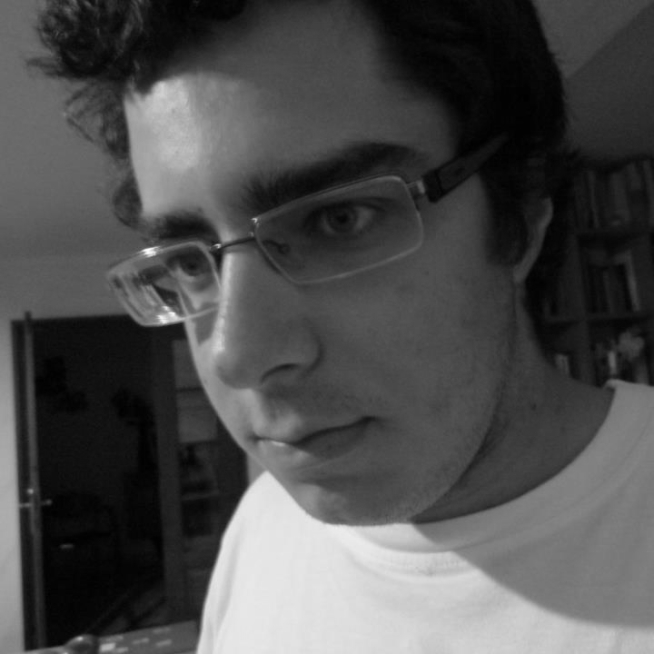
\includegraphics[width=\textwidth]{Santos.jpg}
\end{subfigure}
\end{figure}

\vspace{2cm}
Braga, 1 de junho de 2014

\end{center}

\end{titlepage}
%----------------------------------------------------------------------
\newpage
\phantom{placeholder} % doesn't appear on page
\thispagestyle{empty} % if want no header/footer
%----------------------------------------------------------------------
\tableofcontents
\phantom{placeholder} % doesn't appear on page
\thispagestyle{empty} % if want no header/footer
%----------------------------------------------------------------------
\newpage
\phantom{placeholder} % doesn't appear on page
\thispagestyle{empty} % if want no header/footer
%----------------------------------------------------------------------
\pagestyle{fancy}
\setlength{\headheight}{15.2pt}
\fancyhf{} % apagar as configurações actuais
\fancyfoot[LE,RO]{\thepage}
\fancyhead[LE,RO]{POO --- FitnessUM --- Grupo XXX.}
\setcounter{page}{0}
%----------------------------------------------------------------------

\chapter{Introdução}
\label{cap:intro}
O presente projecto enquadra-se na unidade curricular de Programação Orientada a Objectos do curso de Licenciatura em Engenharia 
Informática da Universidade do Minho.
O projecto pretende implementar uma aplicação, designada \emph{FitnessUM}, para registar e simular actividades desportivas de fitness.
A aplicação pretende foi desenvolvida em \emph{java} e pretende simular um ambiente de rede social.

\section{Objectivos}
\label{sec:obj}
(...)

De acordo com o enunciado \cite{enunciado}, os principais objectivos definidos para a aplicação são os seguintes (\emph{requisitos}):
\begin{itemize}
\item \textbf{req1:} (...);
\item \textbf{req2:} (...); 
\item (...); 
\end{itemize}

\section{Organização do Relatório}
\label{sec:org}
(...)

\chapter{Arquitectura e Descrição da Aplicação}
\label{cap:arq}
\section{Organização de Pastas e Ficheiros}
\label{sec:folders}
(...)
Model–view–controller (MVC) figura \ref{fig:mvc}.
(...)
\begin{figure}
\centering
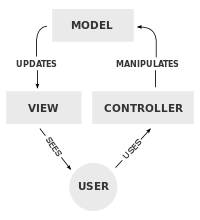
\includegraphics[width=4cm]{MVC-Process.png}
\caption{Diagrama com a relação típica dos componentes do MVC (ref.:\url{http://en.wikipedia.org/wiki/Model-view-controller}).}
\label{fig:mvc}
\end{figure}
(...)

De forma a manter uma estrutura de pastas partilhada entre os autores e um controlo de versões eficaz, 
foi utilizada a ferramenta open source \emph{GIT} (\url{http://git-scm.com/}), 
com repositório privado no bitbucket (\url{https://bitbucket.org/ruiOliveiras94/fitnessum-poo}).

\section{Descrição das Classes}
\label{sec:classes}
(...)
A figura (...) apresenta o grafo de dependências dos vários ficheiros de código, obtido através do \emph{BlueJ}.

\section{Interface com o Utilizador}
\label{sec:interpretador}
(...)

\chapter{Complexidade e Estruturas de Dados}
\label{cap:complexidade}
(...)

\chapter{Cálculo do consumo de calorias por actividade}
\label{cap:calorias}

\chapter{Conclusões}
\label{cap:concl}
(...)

\bibliographystyle{plain}
\bibliography{relatorio-POO-CamposinhosOliveiraSantos}

\appendix
\chapter{Documentação do Código}
\label{anex:doc}

\chapter{Demo da aplicação}
\label{anex:demo}




\end{document}
